
\chapter{The Characterization of a Flash-based Subsystem}

In this chapter, the way OpenFlash model a NAND flash subsystem is presented. OpenFlash models the structure, functions, performance and power consumption behaviors of the NAND subsystem. Understanding the concepts presented in this chapter is essential to efficiently use the API offered by the OpenFlash flash subsystem API. 

\section{General concepts}

OpenFlash implements models to describe a flash subsystem structure and behavior, and compute its performance / power consumption during a simulation. Before a simulation, the user inputs parameter values for these models to describe the desired flash subsystem. OpenFlash implements the following models:
\begin{itemize}
  \item The \emph{structural model} is used to describe the internal architecture of the depicted flash subsystem ;
  \item The \emph{functional model} is used to describe the flash commands supported by the subsystem, and the way these commands are processed ;
  \item The \emph{performance model} is used to compute execution times taken by the different flash event occurring during the simulation, and calculated by the functional model ;
  \item The \emph{power consumption model} is very similar to the performance model, but it targets energy computation.
\end{itemize}

\section{Structural model}

The structural model is used to define the architectural characteristics of the simulated flash subsystem. As OpenFlash targets system level simulation, it does not go deep into the details of the described system. As for the flash subsystem layer, the flash page is the finest level of granularity considered by the software.

\subsection{A flash chip}

\begin{figure}
  \center
  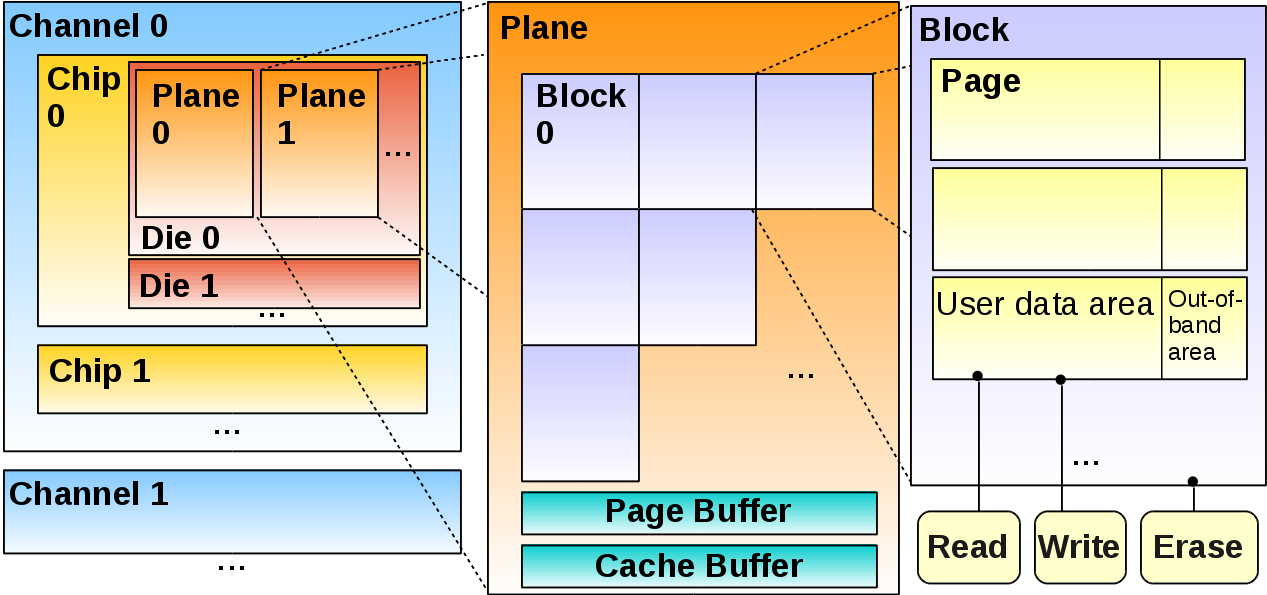
\includegraphics[width=0.95\textwidth]{Includes/ArchFlash_Fat.png}
  \caption{The flash subsystem structure implemented by OpenFlash}
  \label{fig:archflash}
\end{figure}

As depicted on Figure \ref{fig:archflash} page \pageref{fig:archflash}, OpenFlash models the architecture of a NAND flash chip as the organization of hierarchical elements :
\begin{itemize}
  \item A flash \emph{chip} is composed of one or several \emph{dies} ;
  \item A \emph{die} contains one or several \emph{planes} ;
  \item A \emph{plane} contains multiple \emph{blocks}. A plane also contains a \emph{page buffer} used to buffer data read / written during I/O operations. A plane can also contain a \emph{cache buffer} whose goal will be explained in the functional model section ;
  \item A \emph{block} contains multiple \emph{pages} ;
  \item Finally, a \emph{page} is divided between the \emph{user data area} and the \emph{Out-Of-Band} (OOB) area.
\end{itemize}

This structural flash chip model can be illustrated with some real world values. For example, let's take a look at the Micron NAND data-sheet available at the following URL:\\\href{http://download.micron.com/pdf/datasheets/flash/nand/4gb_nand_m40a.pdf}{\textit{http://download.micron.com/pdf/datasheets/flash/nand/4gb\_nand\_m40a.pdf}}.

In this example, the page size is 2048 bytes (user data area) + 64 bytes (OOB). One block contains 64 pages, and one plane contains 2048 blocks. According to the model, one chip can contains 1, 2 or 4 stacked dies. Finally, Each die contains two planes.

As some simple embedded NAND storage subsystems only include one chip, more complex storage subsystems exist. OpenFlash is able to simulate multi-chips, multi-channels storage subsystems like those found in SSDs.

\subsection{Multi-chips, Multi-channels SSD storage subsystem}

SSDs contains several NAND flash chips. Flash chips sharing the same I/O bus are regrouped into channels. A SSD can include multiple channels to perform true parallelism operations. Chips and channels organization are also depicted on Figure \ref{fig:archflash}.

  \section{Functional model}
  
The goal of the functional model is to depict the various operations supported by the flash subsystem. The operation implemented by OpenFlash are divided into four categories. The \emph{legacy operations} are the basic NAND read, write and erase operations supported by all devices. \emph{Intra-chip advanced operations} are supported by some devices and are performed inside one NAND chip. The \emph{intra chip advanced combined operations} are a combination of several operation from the previous categories. Finally, \emph{Multi devices} operations are performed on several chips or channels. Therefore, they are only supported in multi-chip / multi channels storage subsystems like SSDs.

The full list of NAND subsystem operations implemented by OpenFlash is as follows:

\begin{itemize}
  \item \textbf{Legacy operations:}
  \begin{itemize}
    \item \emph{Legacy page read} \& \emph{write}, \emph{legacy block erase} ;
  \end{itemize}
  \item \textbf{Intra-chip advanced operations:}
  \begin{itemize}
    \item \emph{Copy back} or \emph{internal data move} ;
    \item \emph{Cache read} / \emph{write} ;
    \item \emph{Multi plane page read} \& \emph{write}, \emph{multi plane block erase} ;
    \item \emph{Die interleaved page read} \& \emph{write}, \emph{die interleaved block erase} ;
  \end{itemize}
  \item \textbf{Intra-chip advanced combined operations:}
  \begin{itemize}
    \item \emph{Multi plane cache read} \& \emph{write} ;
    \item \emph{Die interleaved cache read} \& \emph{write} ;
    \item \emph{Multi plane copy back} ;
    \item \emph{Die interleaved copy back} ;
    \item \emph{Die interleaved multi plane page read} \& \emph{write}, \emph{die interleaved multi plane block erase} ;
    \item \emph{Die interleaved multi plane cache read} \& \emph{write}
  \end{itemize}
  \item \textbf{Multi devices operations:}
  \begin{itemize}
    \item \emph{Multi chips} commands ;
    \item \emph{Multi channels} commands.
  \end{itemize}
\end{itemize}

In the following sections those operations are depicted in details. Back to our Micron NAND data sheet example, we can see that the described flash chip model supports of course legacy operations. In addition, its supports cache operations, copy back, and multi plane operations, as well as a combination of those advanced commands. Finally, according to the chip model, multiple dies models support die interleaved operations.

For each NAND operation implemented by the OpenFlash flash subsystem layer, we give a description of the operation and a list of the constraints applying to this operation. One obvious constraint which apply to all operation is the fact that the addressed elements (page, block, plane, etc.) must be inside the address range of the described NAND subsystem.

\subsection{Legacy operations}

\subsubsection{Legacy read}
The legacy read command performs a read operation targeting a flash page. It is supported by all flash subsystems. There is no particular constraint for this operation, aside from the fact that the addressed page must be in the address range of the described flash subsystem. A legacy read operation reads the full page, i.e. the user data area \emph{and} the OOB area. Separating the user data from the OOB data is the role of the control layer.

An example of legacy read is illustrated on Figure \ref{fig:archflash} page \pageref{fig:archflash}.

\subsubsection{Legacy write}
The legacy write command performs a write operation on a full page. It is supported by all flash subsystems. The following constraints apply:

\begin{enumerate}
  \item One cannot write in a page already containing data (previously written), the page must first be erased before being re-written ;
  \item Writes in a block should be sequential (i.e. starting from page 0 to the last page of the block) to avoid disturbance. This is a common problem for NAND flash.
\end{enumerate}

The write operation is achieved on a full page and write the user data area and the OOB area. The content of the OOB area is generally determined by the flash control layer based on the user data written and the control layer internal data structures.

An example of legacy write is illustrated on Figure \ref{fig:archflash} page \pageref{fig:archflash}.

The presented write constraints are core constraints of NAND flash memory. They will apply to each advanced operation presented in the remainder of this document.

\subsubsection{Legacy erase}
The erase operation is achieved on a whole block: all the pages contained in the targeted block are erased and become ready to be written. Apart from the address range, no particular constraint apply.

An example of legacy erase is illustrated on Figure \ref{fig:archflash} page \pageref{fig:archflash}.

\subsection{Intra chip advanced operations}

\subsubsection{Copy back}

The copy back operation may be also referred as \emph{internal data move}. It consists in using the page buffer to copy data from a page to another inside one plane, without occupying the I/O bus. The following constraints apply:

\begin{figure}
  \center
  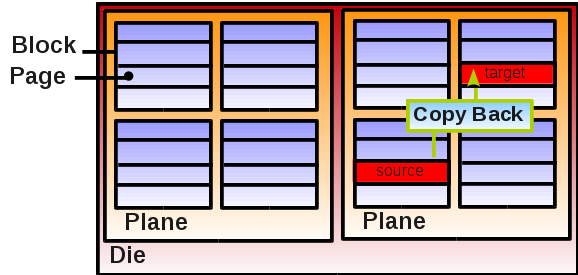
\includegraphics[width=0.5\textwidth]{Includes/CopyBack.png}
  \caption{An example of a copy back operation}
  \label{fig:copyback}
\end{figure}

\begin{enumerate}
  \item The page index in their blocks of the source (read) page and the target (written) page must be both odd or both even ;
  \item Source and target must be in the same plane of a chip ;
  \item Write operation constraints apply on the target page.
\end{enumerate}

An example of copy back operation is illustrated on Figure \ref{fig:copyback}.

\subsubsection{Cache read}
Cache read is an advanced command made possible by the introduction of a cache buffer in addition to the page buffer inside each plane of the NAND chip (see Figure \ref{fig:archflash} page \pageref{fig:archflash}). The cache buffer is connected to the page buffer. It is then possible, when reading several pages from the same block in a sequential way, to pipeline I/O transfers (A) from the NAND array to the page buffer, and (B) from the cache buffer to the I/O bus. This allow to increase the performance of sequential page read operations.

The following constraints apply to the cache read operation:

\begin{enumerate}
  \item The pages must be read in a sequential way ;
  \item The entire set of pages read must not exceed the containing block boundary.
\end{enumerate}

An example of cache read operation is illustrated on the left side of Figure \ref{fig:cacheop}.

\begin{figure}
  \center
  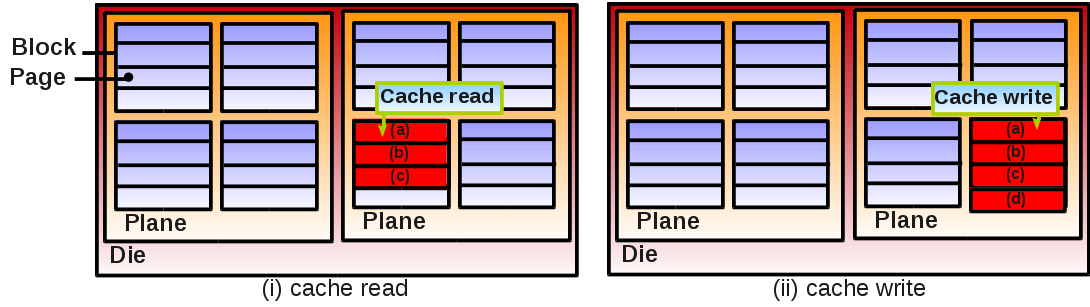
\includegraphics[width=0.99\textwidth]{Includes/CacheOp.png}
  \caption{Examples of cache read (left) and cache write (right) operations}
  \label{fig:cacheop}
\end{figure}

\subsubsection{Cache write}
The cache write operation works the same way as the cache read command. In addition to the previously explained constraints applying to the cache read operation, the cache write command is subject to the write operation constraints: every page in the written set must be free (erased). If the cache write operation starts in a block a an offset different from 0, the pages of index 0 up to that offset must have previously been written to satisfy the constraint saying that writes in a block must always be sequential.

An example of a cache write operation is illustrated on the right side of Figure \ref{fig:cacheop}.

\subsubsection{Multi plane read}

Multi plane read operation allow reading data from pages in different planes of the same die. The transfer between NAND array and the page buffer is realized in parallel in each targeted plane. Strong constraints apply on multi plane read operations (and on multi plane operation in general):

\begin{enumerate}
  \item Targeted pages to read must belong to different planes in the same die ;
  \item The addresses of the pages to read in each plane is represented by a couple (\emph{block index in the plane}, \emph{page index in this block}). All the pages targeted by the multi plane read operation must have the same address couple (\emph{block}, \emph{page}) in the targeted planes ;
  \item The multi plane operation is performed on \emph{all} the planes of the same die.
\end{enumerate}

Examples of a valid multi plane read operation, and an invalid multi plane read operations are presented on the top of Figure \ref{fig:multiplaneop}. On the top left side the multi plane operation is valid because the in-plane address (\emph{block}, \emph{page}) inside each plane of the targeted die is the same. The top right side illustrates a multi plane operation which is not feasible because the addresses inside each plane are different.

\begin{figure}
  \center
  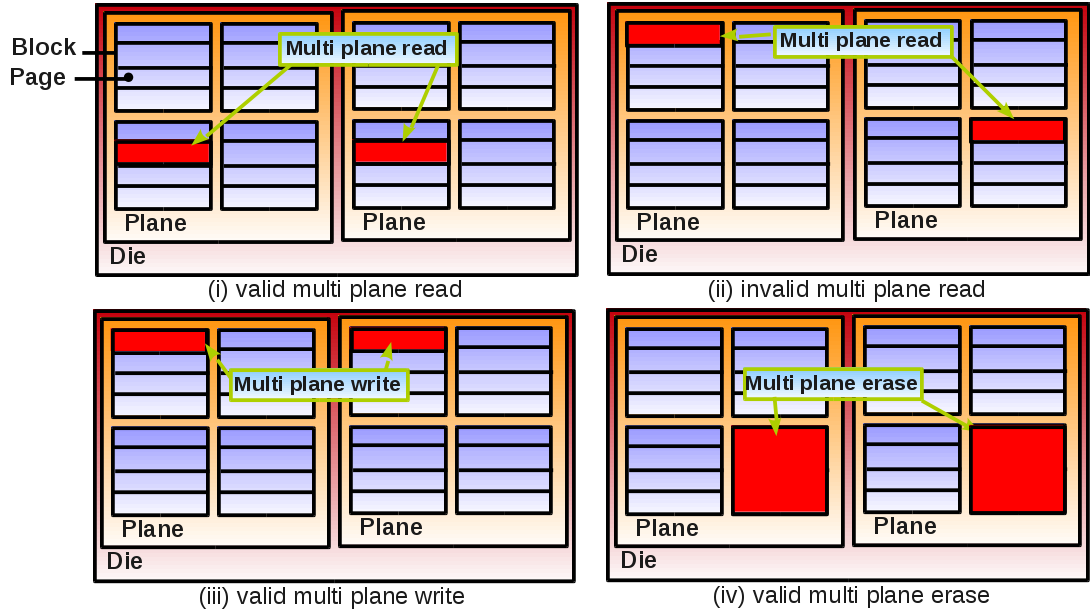
\includegraphics[width=0.9\textwidth]{Includes/MultiPlaneOp.png}
  \caption{Examples of multi plane operations: a valid multi plane read (i), an invalid multi plane read (ii), a valid multi plane write (iii) and a valid multi plane erase (iv).}
  \label{fig:multiplaneop}
\end{figure}

\subsubsection{Multi plane write}
This command is similar to the multi plane read operation, aside from the fact that targeted pages are written. The multi plane operation constraints apply, in addition to the standard write constraints:

\begin{enumerate}
  \item Targeted pages to write must belong to different planes in the same die ;
  \item The addresses of the pages to write in each plane is represented by a couple (\emph{block index in the plane}, \emph{page index in this block}). All the pages targeted by the multi plane write operation must have the same address couple (\emph{block}, \emph{page}) in the targeted planes ;
  \item The multi plane operation is performed on \emph{all} the planes of the same die ;
  \item Writes must occur on free pages, and writes in each block must be sequential. For example if a multi plane write operation targets the second page of the first block in each plane of a die, one must ensure that the first page of each block of those planes has previously been written.
\end{enumerate}

On the bottom left of Figure \ref{fig:multiplaneop}, a multi plane write operation is illustrated.

\subsubsection{Multi plane erase}
Multi plane erase allow erasing in parallel several blocks, each one in a different plane of the same die. Multi plane constraints apply:

\begin{enumerate}
  \item Targeted blocks must belong to different planes of the same die ;
  \item The targeted block addresses (i.e. their index in each plane) must all be equal ;
  \item Multi plane erase operation is performed on \emph{all} the planes of the same die ;
\end{enumerate}

On the bottom right of Figure \ref{fig:multiplaneop}, a multi plane erase operation is illustrated.

\subsubsection{Die interleaved read}
The die interleaved read command allows reading in parallel several pages, each one belonging to a different die of the same chip. Unlike the multi plane commands, there is no particular constraint on the page address inside each targeted die. Moreover, the set of targeted die can be a subset of the total number of dies present in the chip.

The following constraints apply on the die interleaved read command:

\begin{enumerate}
  \item Each targeted page must belong to a different die of the same chip.
\end{enumerate}

A die interleaved read operation is illustrated on Figure \ref{fig:dieinterleavedop}.

\begin{figure}
  \center
  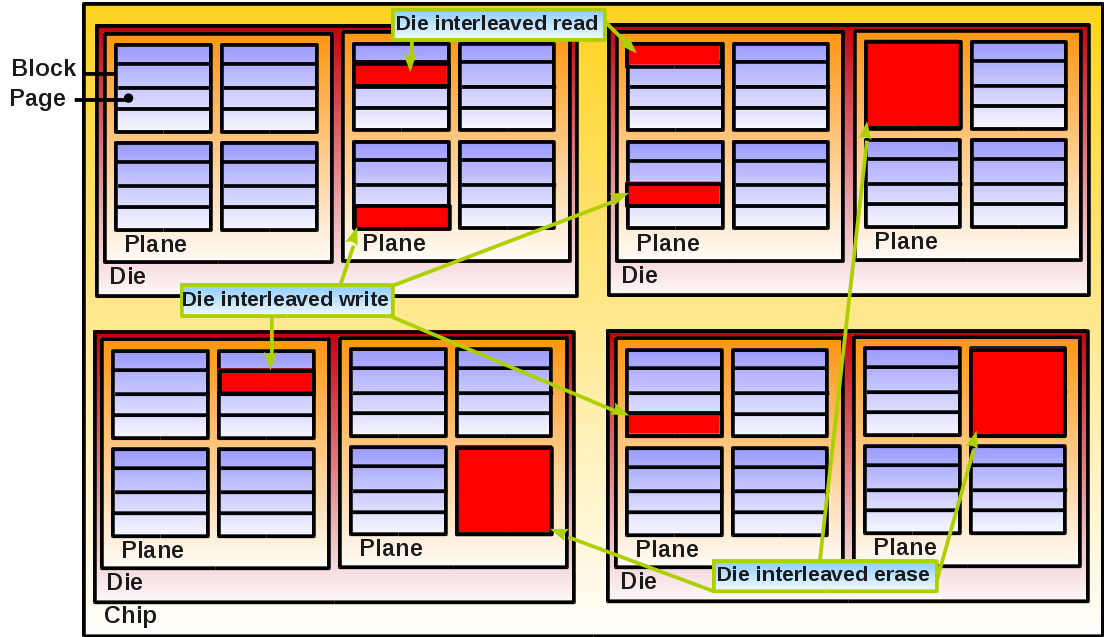
\includegraphics[width=0.9\textwidth]{Includes/DieInterleavedOp.png}
  \caption{Examples of die interleaved read, write and erase operations}
  \label{fig:dieinterleavedop}
\end{figure}

\subsubsection{Die interleaved write}
Die interleaved write command works in a similar way to the die interleaved read command, but performs write operation. The standard write constraints apply. Thus, die interleaved write constraints are:

\begin{enumerate}
  \item Each targeted page must belong to a different die of the same chip ;
  \item Writes must target free pages and writes in each blocks must be sequential.
\end{enumerate}

An example of die interleaved write operation is presented on Figure \ref{fig:dieinterleavedop}.

\subsubsection{Die interleaved erase}
Die interleaved erase operation does not present any particular constraint, apart from the fact that each targeted block must be located in a different die of the same chip.

An example of die interleaved erase operation is presented on Figure \ref{fig:dieinterleavedop}.

\subsection{Intra chip advanced combined operations}
Those commands are a combination of the previously presented advanced commands.

\subsubsection{Multi plane cache operations}
Multi plane cache read and multi plane cache write operation allow reading / writing sets of pages sequentially in all the planes of the same die. Constraints for the multi plane operations \emph{and} the cache read / write operation apply.

The constraint on a multi plane cache read operation are the following:

\begin{enumerate}
  \item Each set of pages read must be in the same location in each plane of the die targeted by the operation ;
  \item Each set of pages read must be in a different plane of the same die ;
  \item The operation must target all the planes of the same die ;
  \item Pages must be read in each plane in a sequential way ;
  \item The sets must not exceed the containing block boundary ;
\end{enumerate}

The multi plane cache write operation exhibits the same constraints, with the addition of the standard write constraints: each page written must be free, and writes must occur sequentially in a block.

Examples of multi plane cache read and write operations are presented on Figure \ref{fig:multiplanecacheop}.

\begin{figure}
  \center
  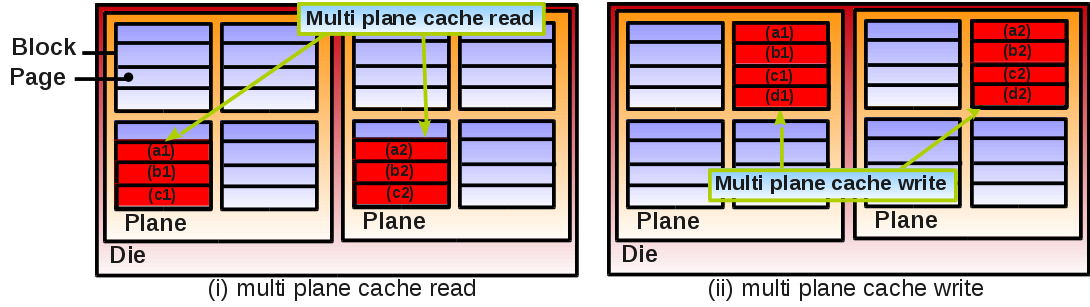
\includegraphics[width=0.9\textwidth]{Includes/MultiPlaneCacheOp.png}
  \caption{Examples of multi plane cache read (left) and multi plane cache write (right) operations}
  \label{fig:multiplanecacheop}
\end{figure}

\subsubsection{Die interleaved cache operation}
Die interleaved cache read and write operations allows performing multiple cache read or multiple cache write in different dies of the same chip. Cache read and write operation constraints apply. As compared to the multi plane cache operations, the sets read / written during die interleaved cache read / write can be at different location within the targeted dies, and of different sizes. Moreover, it is not mandatory to target \emph{all} the dies in the chip.

The following constraints apply to the die interleaved cache read operation:

\begin{enumerate}
  \item Each set of pages read must be in a different die of the same chip ;
  \item Pages in a set must be read sequentially ;
  \item The sets must not exceed the containing block boundary ;
\end{enumerate}

For the die interleaved cache write command, the standard write constraints apply: pages written must be free, and writes must occur sequentially within a block.

Examples of die interleaved cache read and die interleaved cache write operations are illustrated on figure \ref{fig:dieinterleavedcacheop}.

\begin{figure}
  \center
  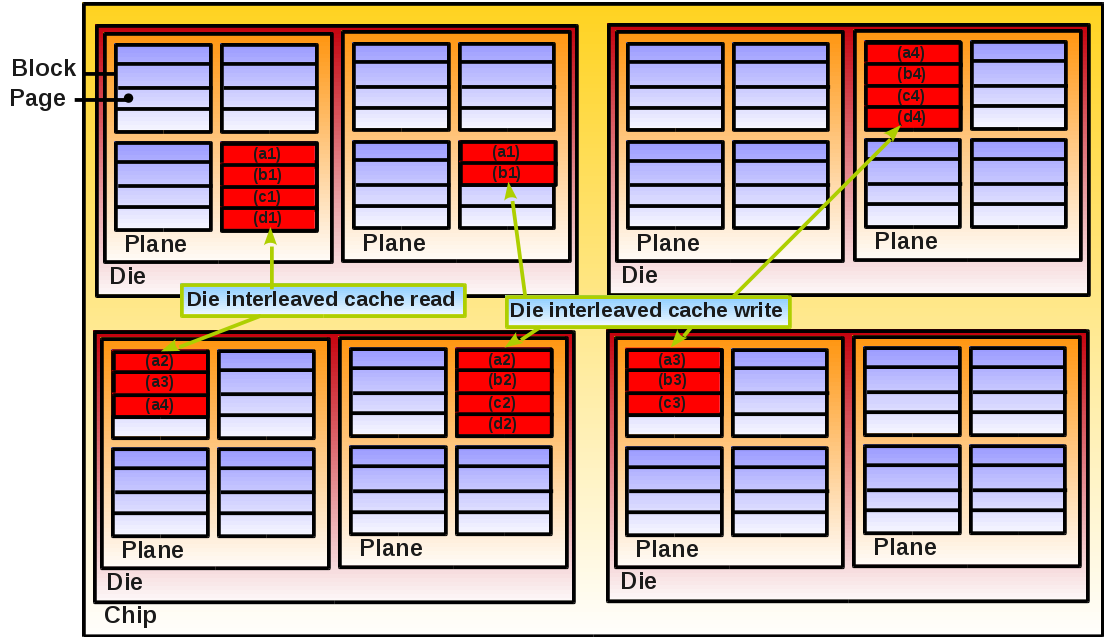
\includegraphics[width=0.9\textwidth]{Includes/DieInterleavedCacheOp}
  \caption{Examples of die interleaved cache read and die interleaved cache write operations}
  \label{fig:dieinterleavedcacheop}
\end{figure}

\subsubsection{Multi plane copy back}
This operation allow performing several copy back operation in each plane of the same die. The multi plane constraint apply: the addresses for source and target pages must be the same in each plane of the targeted die. Source and target index within their containing block must be both odd, or both even (copy back constraint).

To summarize the multi plane copy back constraints :

\begin{enumerate}
  \item Each copy back operation must be performed in a different plane of the same die ;
  \item Sources pages for the set of copy back executed must have the same address (\emph{block}, \emph{page}) within each plane ; 
  \item Target pages must also have the same address (\emph{block}, \emph{page}) within each plane ;
  \item Copy back operations are executed in \emph{all} the planes of the targeted die ;
  \item The in-block index of target and source pages of each copy back operation must be both odd or both even.
  \item Standard write constraints apply on the target page of each copy back operation: it must be free and write in the containing block must occur sequentially.
\end{enumerate}

An example of a multi plane copy back operation is illustrated on Figure \ref{fig:combinedcopyback}.

\subsubsection{Die interleaved copy back}

The die interleaved copy back perform several copy back operation in parallel, in different dies of the same chip. As with all the die interleaved operations, it is not mandatory to target \emph{all} the dies in each chip. There is also no constraint on the address of the copy back operations (apart from the constraint relative to the copy back operations themselves).

The following constraint apply:

\begin{enumerate}
  \item Each copy back operation must be in different dies of the same chip ;
  \item The in-block index of target and source pages of each copy back operation must be both odd or both even.
  \item Standard write constraints apply on the target page of each copy back operation: it must be free and write in the containing block must occur sequentially.
\end{enumerate}

An example of a die interleaved copy back operation is illustrated on Figure \ref{fig:combinedcopyback}.

\begin{figure}
  \center
  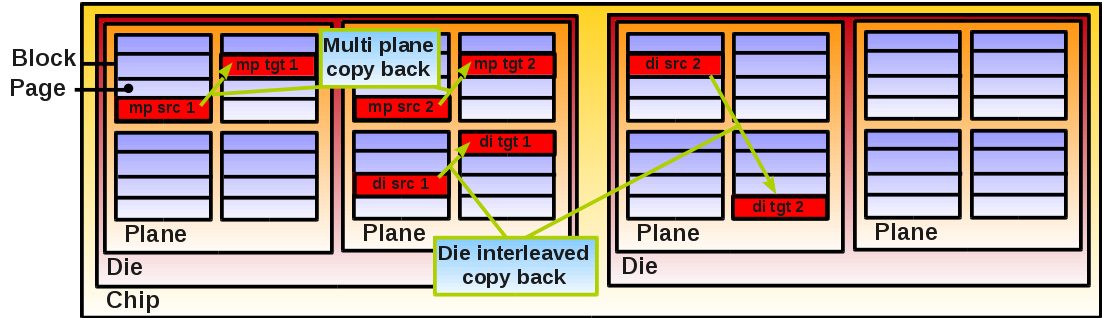
\includegraphics[width=0.9\textwidth]{Includes/CombinedCopyBack.png}
  \caption{Examples of multi plane copy back and die interleaved copy back operations}
  \label{fig:combinedcopyback}
\end{figure}

\subsubsection{Die interleaved multi plane read / write / erase operations}
These operation are used to launch several multi plane page read / write and multiple multi plane block erase in several dies of the same chip.

Each page read / write / block erase multi plane operation must satisfy the related constraints mentioned above. Multi plane read / write / erase launched in different dies can be at various addresses.

Examples of die interleaved multi plane read / write / erase operations are illustrated on Figure \ref{fig:dieinterleavedmultiplaneop}.

\begin{figure}
  \center
  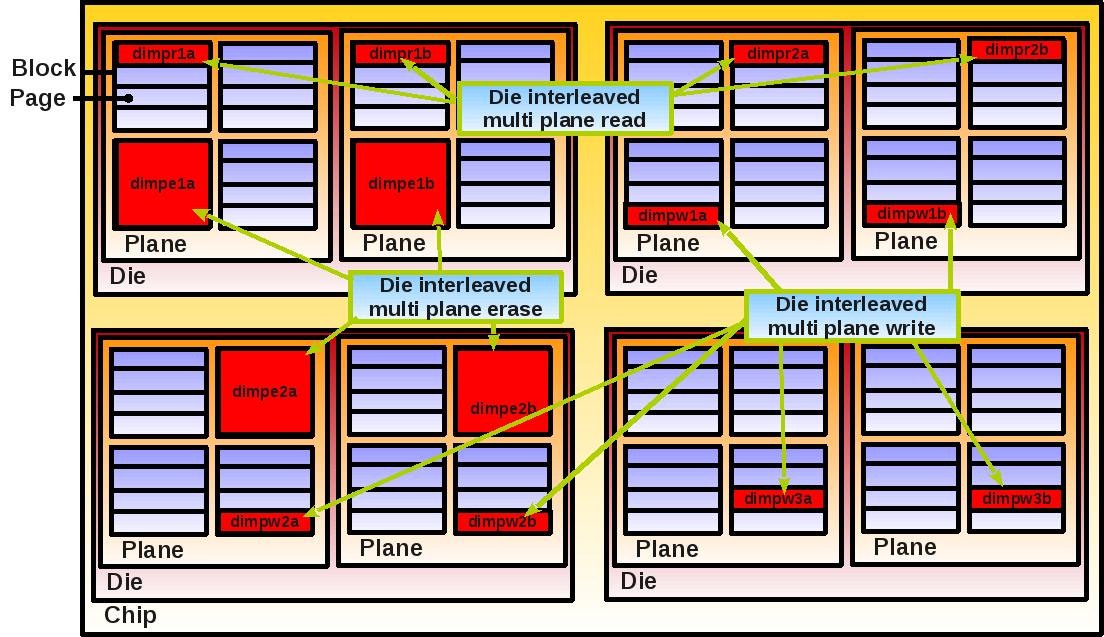
\includegraphics[width=0.9\textwidth]{Includes/DieInterleavedMultiPlaneOp.png}
  \caption{Example of die interleaved multi plane read / write / erase operations}
  \label{fig:dieinterleavedmultiplaneop}
\end{figure}

\subsubsection{Die interleaved multi plane cache operation}
These commands allow launching several multi plane cache read / write operation in different dies of the same chip. Each multi plane cache read / write operation launched in a die must satisfy the constraints of multi plane cache read / write operations. Between different dies, multi plane cache operations can target different addresses and be of various sizes (int terms of number of pages read / written in cache mode).

\begin{figure}
  \center
  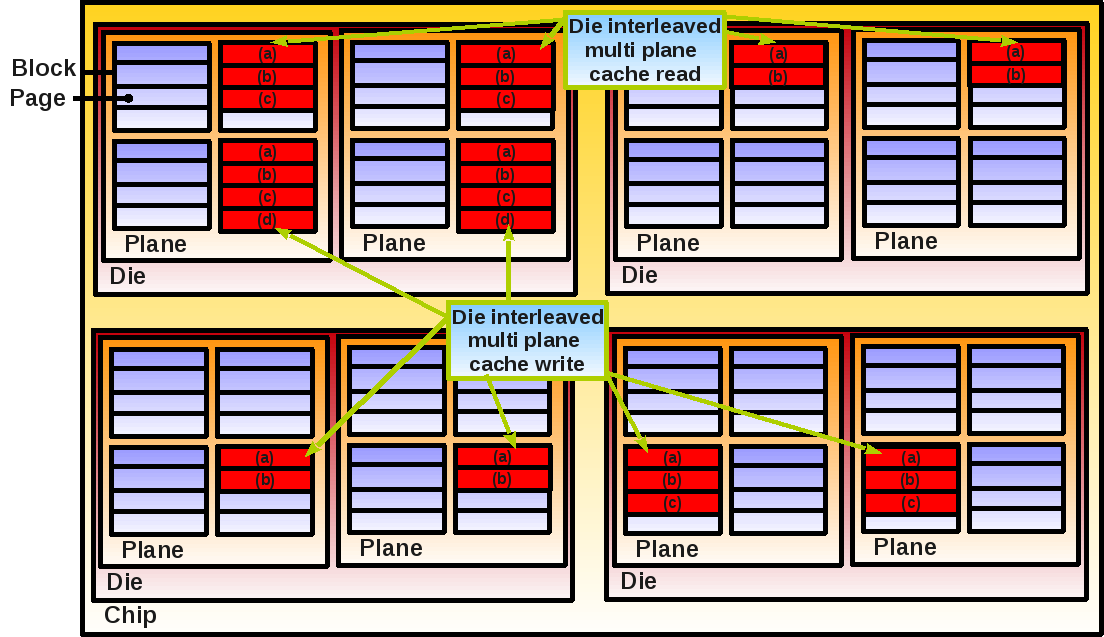
\includegraphics[width=0.9\textwidth]{Includes/DieInterleavedMultiPlaneCacheOp.png}
  \caption{Example of die interleaved multi plane cache read and write operations}
  \label{fig:dieinterleavedmultiplanecacheop}
\end{figure}

\subsection{Multi devices operations}

\subsubsection{Multi chip}
A multi chip operation allows launching in parallel several NAND commands in several chips in the same channel. Chips in a channel share the same I/O bus. Thus, command opcode, address(es), and potential data are sent on the channel in an interleaved way. The commands are executed in parallel, then potential data are dent back on the I/O bus in an interleaved way.

A multi chip operation can be a set of any of the previously presented commands.
  
\subsubsection{Multi channel}
Multi channel operations allow launching several NAND commands on multiple channels. This allow complex NAND subsystems to offer true parallelism. A multi channel operation can be a set of any of the previously presented commands, including multi chip operations.

\section{Performance model}
The performance model defines the way OpenFlash computes execution times for the various flash events occurring in the simulated NAND subsystem. Flash events are in fact the reception of commands by the subsystem, so the performance model is used to compute the execution times of all the commands supported by the simulated subsystem.

The performance model is a set of equations or functions. Each one is used to compute the execution time of a flash command, according to some meaningful parameters. A simple performance model for a simple NAND subsystem supporting only legacy operations can be illustrated as follows :

\begin{itemize}
  \item $T_{LegacyRead} = 25~\mu$s ;
  \item $T_{LegacyWrite} = 200~\mu$s ;
  \item $T_{LegacyErase} = 1500~\mu$s.
\end{itemize}

With such a performance model we can describe that a legacy page read operation takes 25 $\mu$s, a page write takes 200 $\mu$s, and a block erase 1500 $\mu$s. The same performance model can be represented as a set of C++ function as follows:

\begin{lstlisting}
double legacyRead()
{
  return 25;
}

double legacyWrite()
{
  return 200;
}

double legacyErase()
{
  return 1500;
}
\end{lstlisting}

For the rest of this document we will present some examples of performance model as C++ functions, because (1) it is the programming language in which OpenFlash is written and (2) mathematical equation can easily be represented as functions. We can describe some more complex performance models that do not return constants but compute their return values based on some parameters :

\begin{lstlisting}
double legacyRead(int AddressedPageIndex)
{
  if(AddressedPageIndex % 2 == 0)
    return 25;
  else
    return 250;
}

double legacyWrite(int AddressedPageIndex)
{
  if(AddressedPageIndex % 2 == 0)
    return 200;
  else
    return 500;
}

double legacyErase()
{
  return 1500;
}

\end{lstlisting}

Here we can see that the time taken to read or write a page is computed according to the address of the targeted page.

\begin{lstlisting}

double copyBack(int sourceIndex, int targetIndex)
{
  double res;
  
  res = legacyRead(sourceIndex) + legacyWrite(targetIndex) - copyBackBenefit;
  
  return res;
}

double dieInterleavedRead(vector<int> pagesToRead)
{
  for(int i=0; i<(int)pagesToRead.size(); i++)
}
\end{lstlisting}

\colorbox{red}{TODO: A completer. Peut etre ne presenter que des concepts theoriques ici}\\
\colorbox{red}{et deplacer tout ce qui \\est code C++ / implementation dans la partie "using the API".}
  
  \section{Power consumption model}

\colorbox{red}{TODO}
